\textbf{/F60/} \\
\textbf{Prozess:} Gemeinsames Losgehen \\
\textbf{Ziel:} Gruppe geht gemeinsam los \\
\textbf{Kategorie:} primär \\
\textbf{Vorbedingung:} Alle Benutzer sind Mitglieder der selben Gruppe \\
\textbf{Nachbedingung (Erfolg):} Mehrere Gruppenmitglieder gehen als Gruppe los\\
\textbf{Nachbedingung (Fehlschlag):} Die Gruppenmitglieder gehen nicht gemeinsam los\\
\textbf{Akteure:} Gruppenmitglieder \\
\textbf{Auslösendes Ereignis:} Ein Gruppenmitglied drückt auf den Go-Button\\
\textbf{Beschreibung:}
\begin{enumerate}
\setlength{\itemsep}{0pt}
\item Ein Gruppenmitglied drückt auf den Go-Button.
\item Der Standort der Person wird zum Server übertragen.
\item Der Standort wird zu allen Gruppenmitgliedern übertragen.
\item Auf einer Karte wird die Position der Gruppenmitglieder angezeigt.
\end{enumerate}

%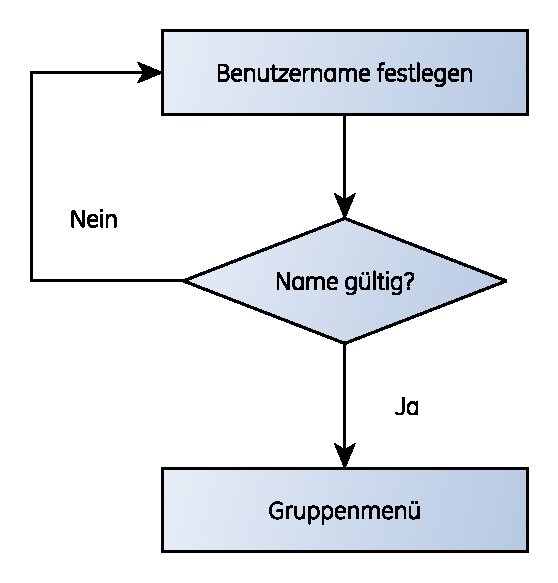
\includegraphics[scale=0.8]{erstmaliges-starten.pdf}
